\newpage
\section{\Large{Use cases}}

\begin{enumerate}[label=\arabic*]
    \item Login
          \begin{enumerate}
              \item When user starts 'TempoMate' app, he can see the login page first. \\
              \item He has three choices, 'Sign in' within the app, 'Continue with Google'. \\
              \item If he choose 'Sign in' within the app, he should enter his ID and password. \\
              \item When login is done successfully, the page turns to the device page. \\
          \end{enumerate}

    \item Signup
          \begin{enumerate}
              \item If user doesn't have his account of signin, he has to create one. \\
              \item After he chooses 'Sign in' at the login page, he clicks the Sign up button. \\
              \item User must enter his ID, password, and password comfirmation to sign up for membership. \\
              \item When he clicks the 'Sign up' button, a account is successfully created. \\
          \end{enumerate}

    \item Logout
          \begin{enumerate}
              \item To log out, user has to go to 'settings' window.\\
              \item If they click the 'Logout' button, it is completed successfully.\\
          \end{enumerate}
\end{enumerate}

\newpage
\begin{enumerate}
    \item Scenario 1 \\
          The first scenario is to set up a 'sleeping routine' for the user to lie in bed and then turn off the lights after 5 seconds.\\
          \begin{enumerate}
              \item User should first add a switch device from the device page. \\
                    \begin{figure}[hbt!]
                        \centering
                        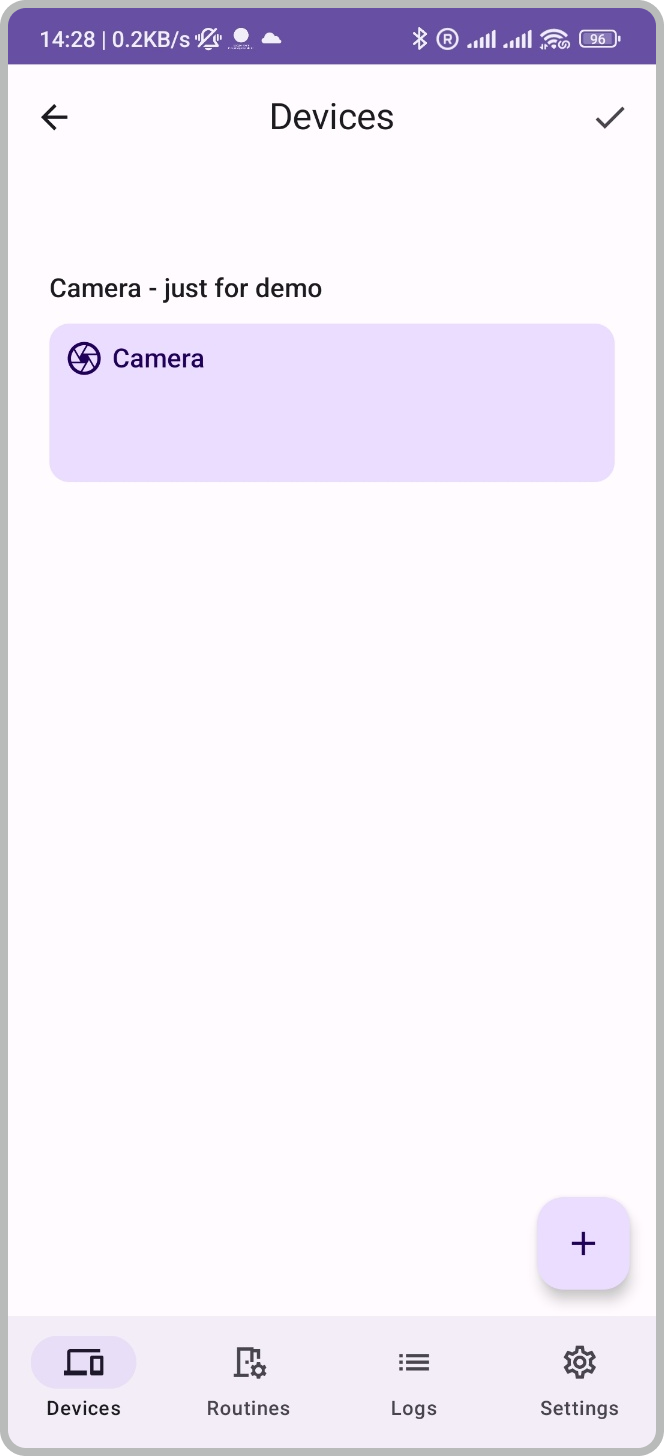
\includegraphics[width=0.5\linewidth]{imgs/usercase/usercase_scenario1_1.png}
                        \caption{Scenario 1.a}
                    \end{figure}
              \newpage
              \item By clicking the plus button on the device page, user can register desired device in the app by scanning the qr code or entering a pairing code.\\
                    \begin{figure}[hbt!]
                        \centering
                        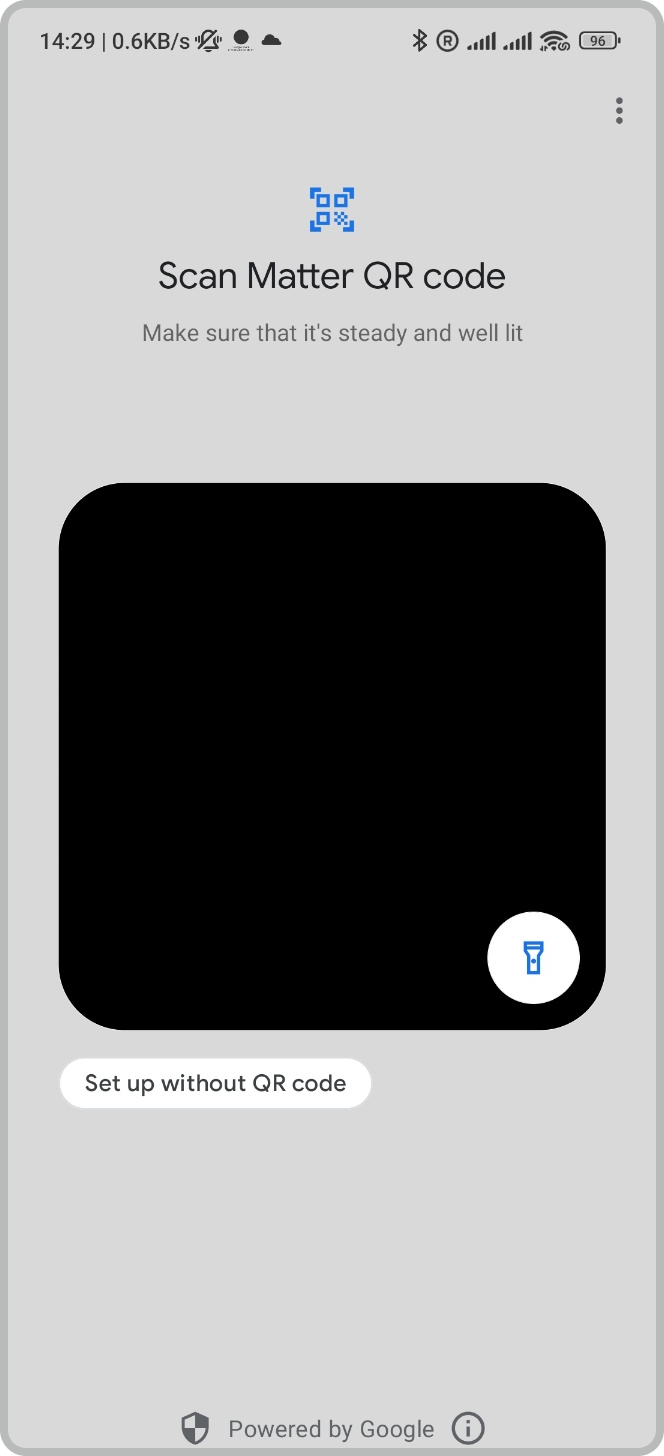
\includegraphics[width=0.5\linewidth]{imgs/usercase/usercase_scenario1_2.png}
                        \caption{Scenario 1.b}
                    \end{figure}
              \newpage
              \item If the connection of the device is successful, the device setup screen appears.\\
                    \begin{figure}[hbt!]
                        \centering
                        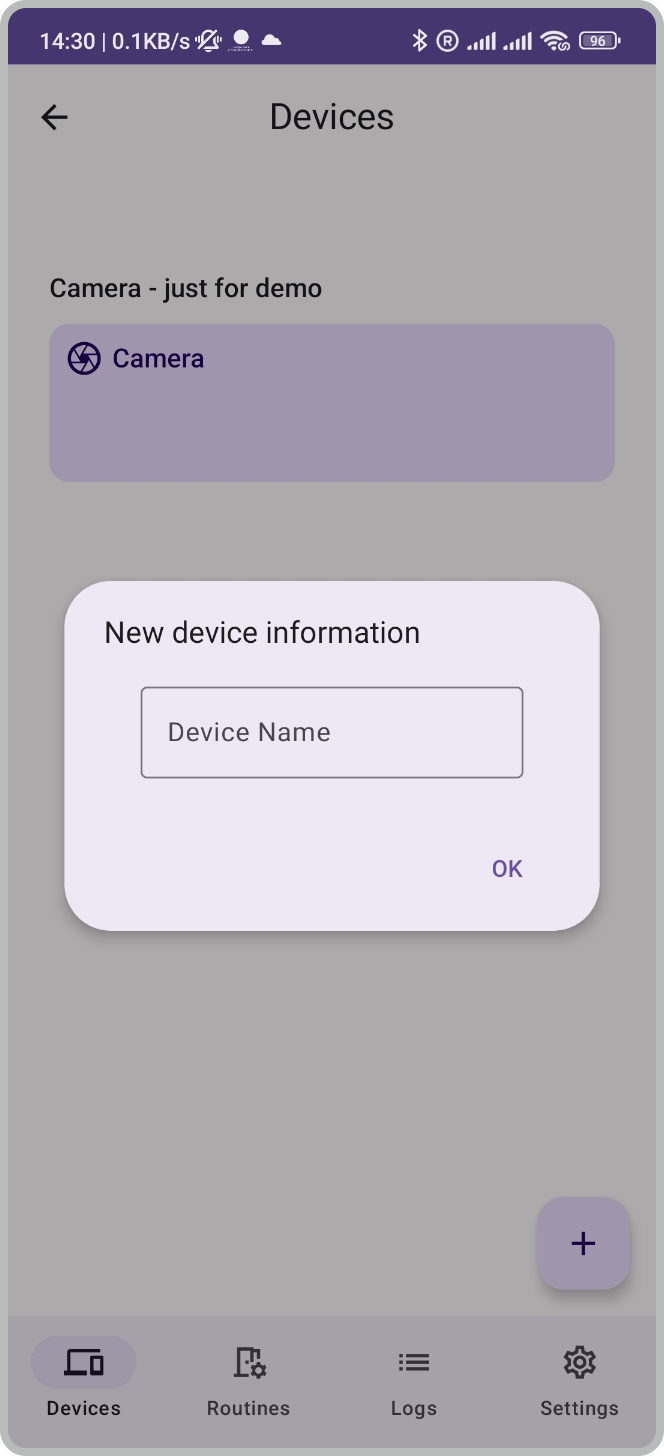
\includegraphics[width=0.5\linewidth]{imgs/usercase/usercase_scenario1_3.png}
                        \caption{Scenario 1.c}
                    \end{figure}
              \newpage
              \item User can press the plus button at the bottom right of the routine page, and enter 'sleeping routine' when the routine name input window appears. \\
              \item Then, the window turns to the routine setting page.\\
              \item User must set trigger for the routine. \\
              \item After user presses the posture trigger button and selects the bedroom camera, he sets the position of the camera to the bed. \\
              \item Next, trigger setting is completed by selecting lie button among sit, stand, and lie to set the lying posture to trigger.\\
                    \begin{figure}[hbt!]
                        \centering
                        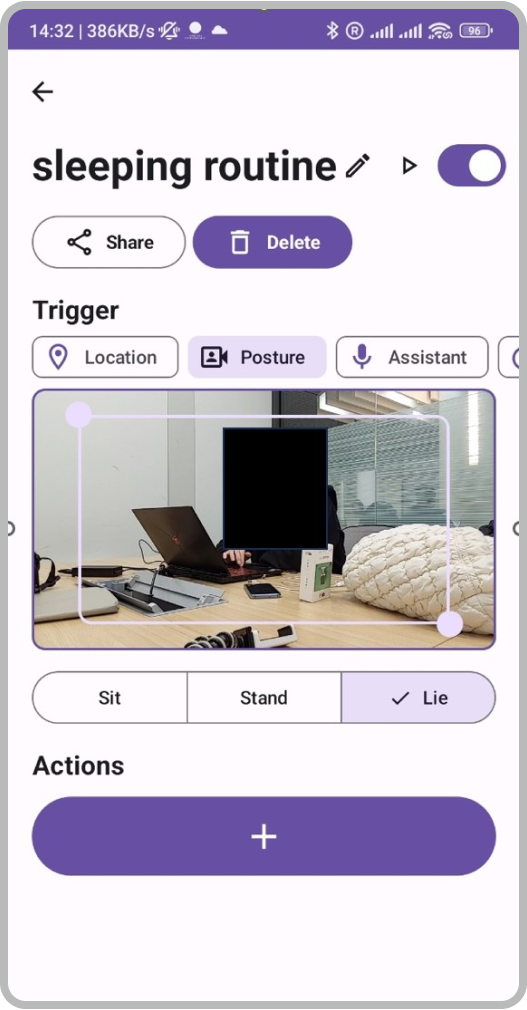
\includegraphics[width=0.5\linewidth]{imgs/usercase/usercase_scenario1_8.png}
                        \caption{Scenario 1.h}
                    \end{figure}
              \newpage
              \item Then, user have to set the actions. \\
              \item User can add several actions through the plus button at the bottom of the page. \\
              \item He should first press the time delay button to set the delay of 5 seconds after lying in bed and set the time delay to 5 seconds. \\
              \item Then, user presses the control device button to select a switch device so that the action of turning off the light is performed, clicks the 'off' button among 'on/off', and finishes adding the action.\\
                    \begin{figure}[hbt!]
                        \centering
                        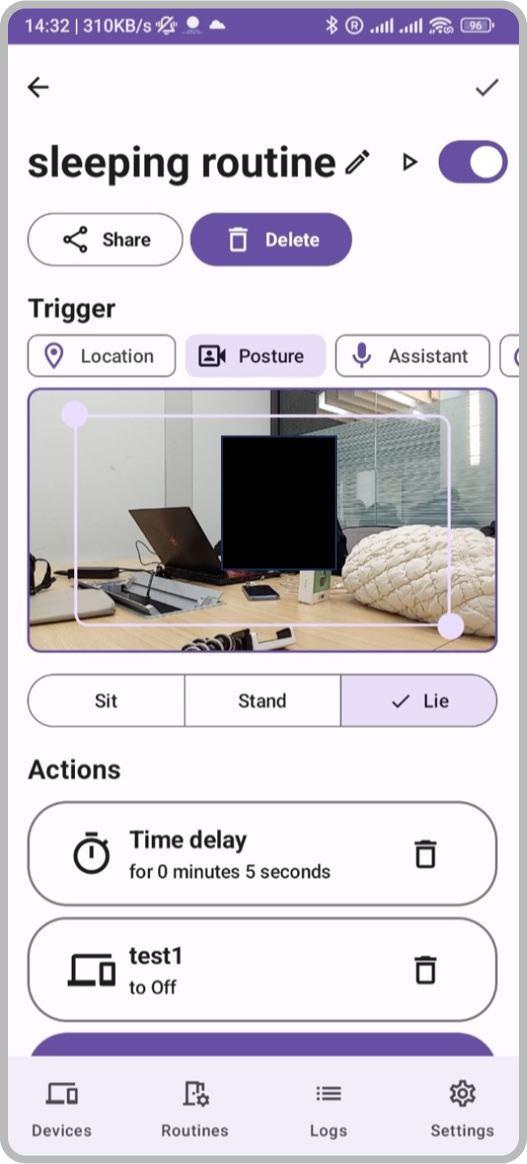
\includegraphics[width=0.5\linewidth]{imgs/usercase/usercase_scenario1_12.png}
                        \caption{Scenario 1.l}                        
                    \end{figure}
              \newpage
              \item Now, the 'sleeping routine' is created. Five seconds after the user lies on the bed in the bedroom, the 'sleeping route' will be executed.\\
                    \begin{figure}[hbt!]
                        \centering
                        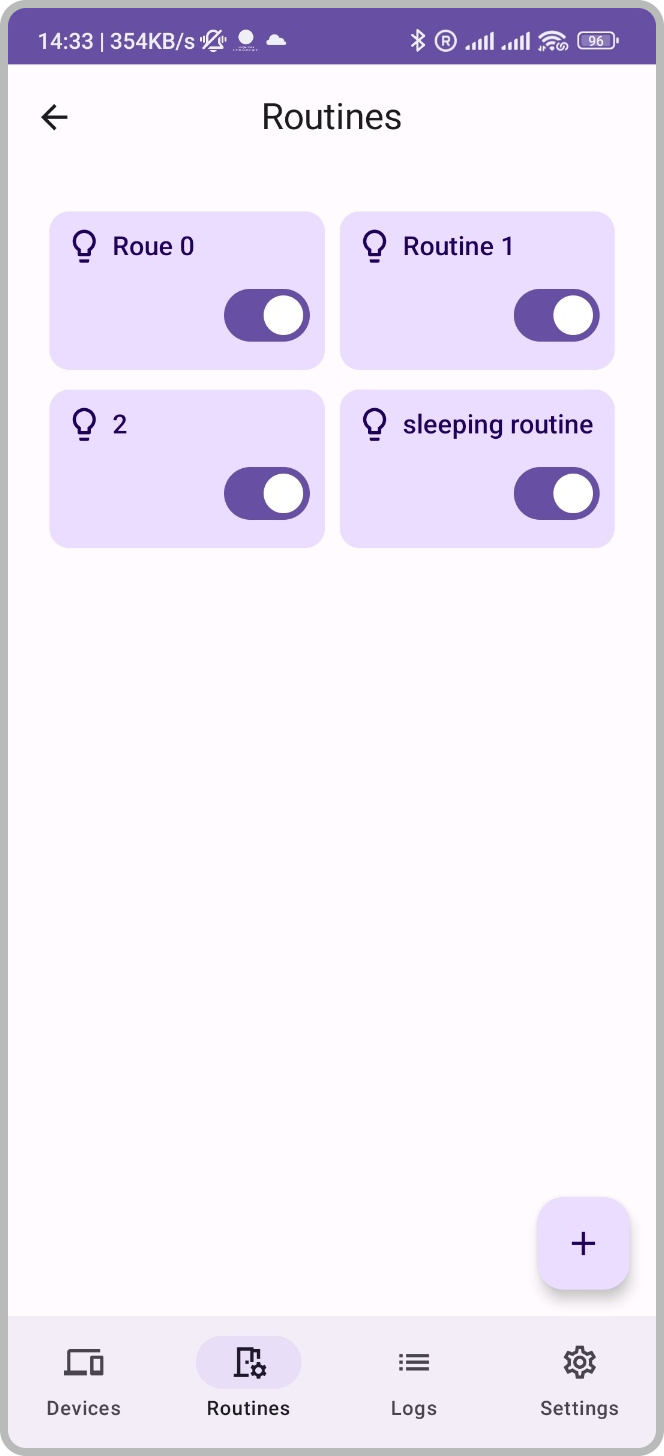
\includegraphics[width=0.5\linewidth]{imgs/usercase/usercase_scenario1_13.png}
                        \caption{Scenario 1.m}                        
                    \end{figure}
          \end{enumerate}
          \newpage

    \item Scenario 2\\
          The second scenario is to rename the 'sleeping routine' to 'night routine' and modify this routine to turn on the TV after the light turns off.\\
          \begin{enumerate}
              \item User has to click the 'sleeping routine' on the routine window. \\
                    \begin{figure}[hbt!]
                        \centering
                        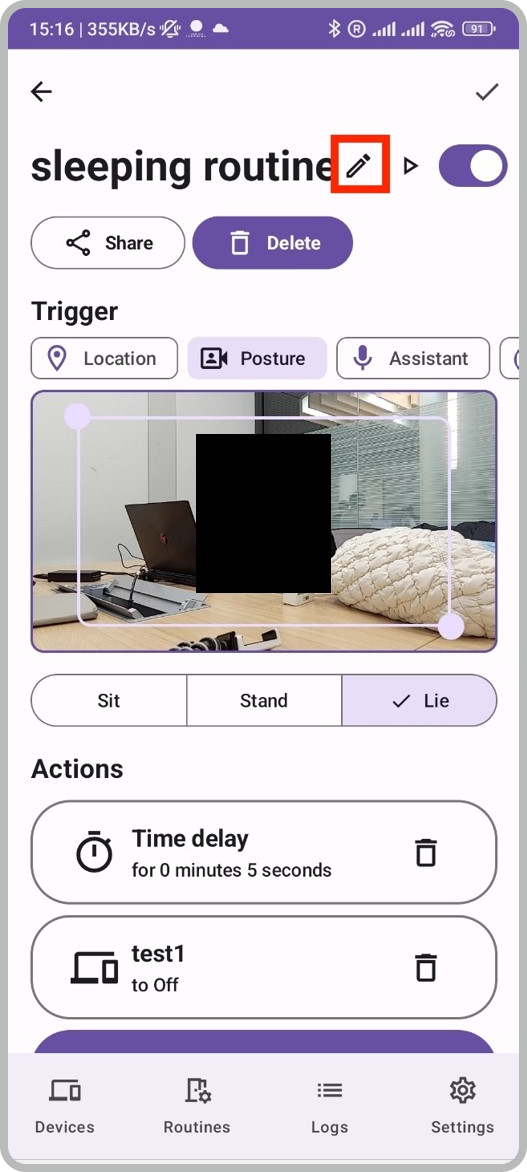
\includegraphics[width=0.5\linewidth]{imgs/usercase/scnario2-1.png}
                        \caption{scenario 2.b}                        
                    \end{figure}
              \newpage
              \item He can see pencil icon next to the routine name 'sleeping routine'. \\
              \item He can clicks this icon and rename the routine name to 'night routine'.\\
              \item Then, user adds TV on action, and click the 'check' button. \\
              \item Modification of the routine is completed. \\
                    \begin{figure}[hbt!]
                        \centering
                        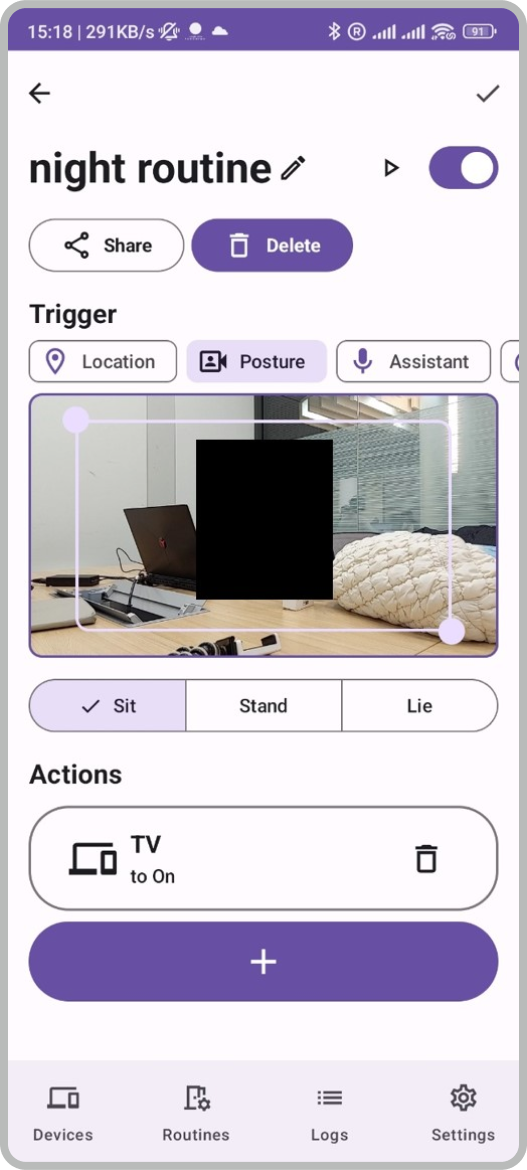
\includegraphics[width=0.5\linewidth]{imgs/usercase/scnario2-2.png}
                        \caption{Scenario 2.e}                        
                    \end{figure}
          \end{enumerate}
          \newpage

    \item Scenario 3\\
          The third scenario is to delete the 5-second delay action of 'night routine'.\\
          \begin{enumerate}
              \item User has to click 'night routine' on the routine window.\\
              \item Then, click the trash can icon next to the 'Time Delay for 5 seconds' action.\\
                    \begin{figure}[hbt!]
                        \centering
                        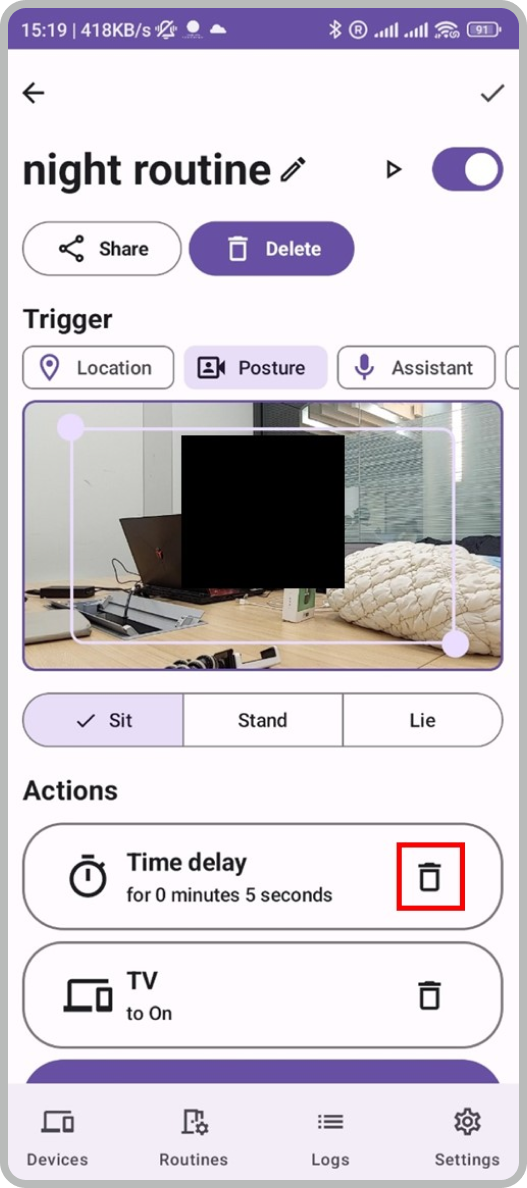
\includegraphics[width=0.5\linewidth]{imgs/usercase/scenario3-b.png}
                        \caption{scenario 3.b}                        
                    \end{figure}
              \newpage
              \item Deletion of this action is completed.\\
                    \begin{figure}[hbt!]
                        \centering
                        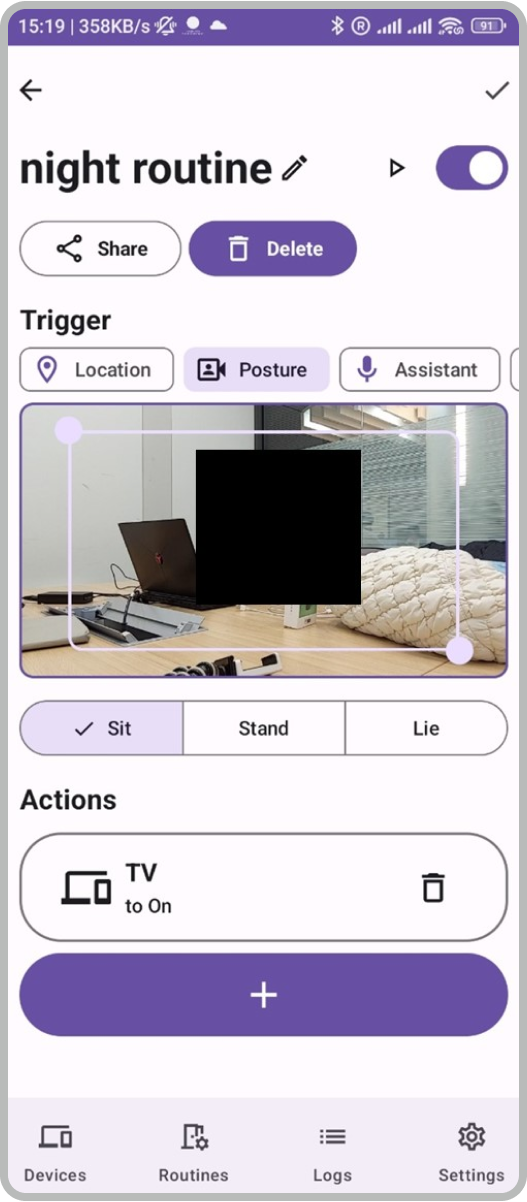
\includegraphics[width=0.5\linewidth]{imgs/usercase/scenario3-c.png}
                        \caption{Scenario 3.c}                        
                    \end{figure}
          \end{enumerate}
          \newpage

    \item Scenario 4\\
          The fourth scenario is to delete the 'night routine'.\\
          \begin{enumerate}
              \item To delete the routine, user has to click the 'night routine' on the routine window.\\
              \item User can see 'Share' and 'Delete' buttons above.\\
                    \begin{figure}[hbt!]
                        \centering
                        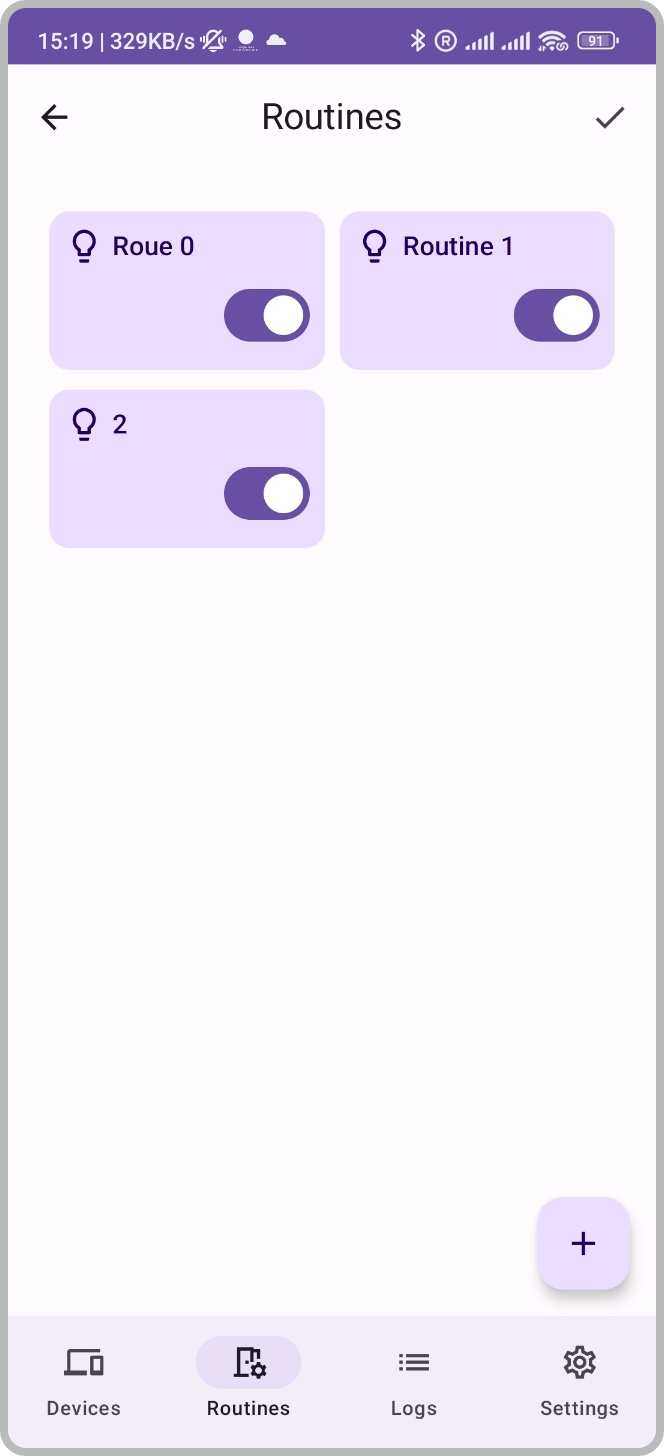
\includegraphics[width=0.5\linewidth]{imgs/usercase/scenario4-b.png}
                        \caption{Scenario 4.b}                        
                    \end{figure}
              \newpage
              \item When he clicks the 'Delete' button, this routine is successfully deleted.\\
                    \begin{figure}[hbt!]
                        \centering
                        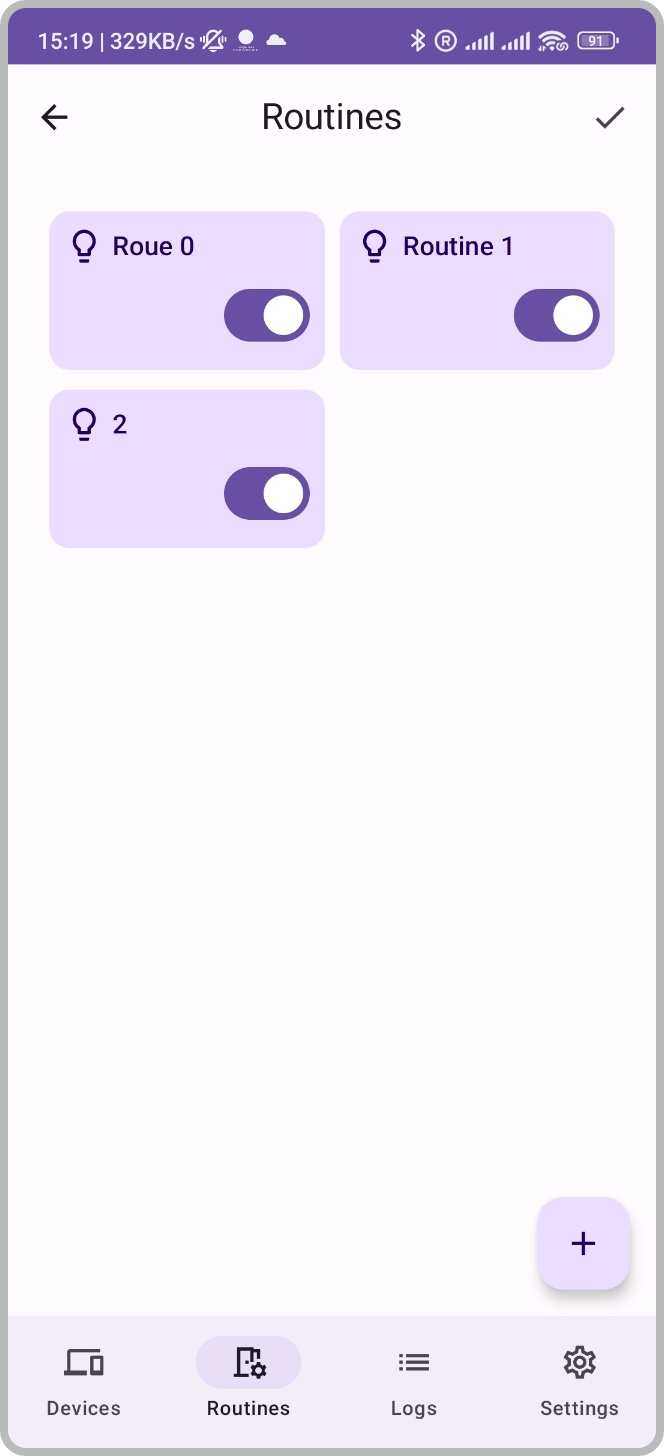
\includegraphics[width=0.5\linewidth]{imgs/usercase/scenario4-c.png}
                        \caption{Scenario 4.c}                        
                    \end{figure}
          \end{enumerate}
          \newpage

    \item Scenario 5\\
          The fifth scenario is to turn off the push notification of the start of the routine.\\
          \begin{enumerate}
              \item First, user has to click 'settings' button to bring up the setting page.\\
                    \begin{figure}[hbt!]
                        \centering
                        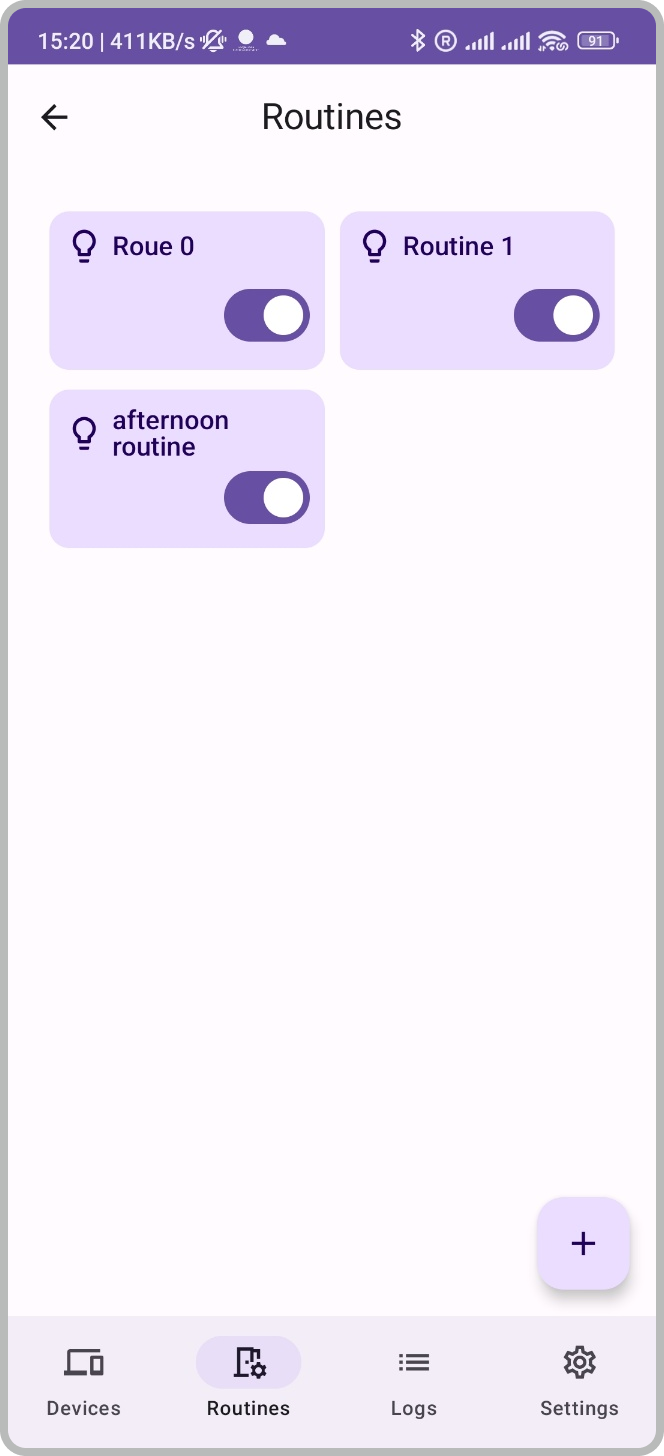
\includegraphics[width=0.5\linewidth]{imgs/usercase/scenario6-a.png}
                        \caption{Scenario 6.c}                        
                    \end{figure}
                    \begin{figure}[hbt!]
                        \centering
                        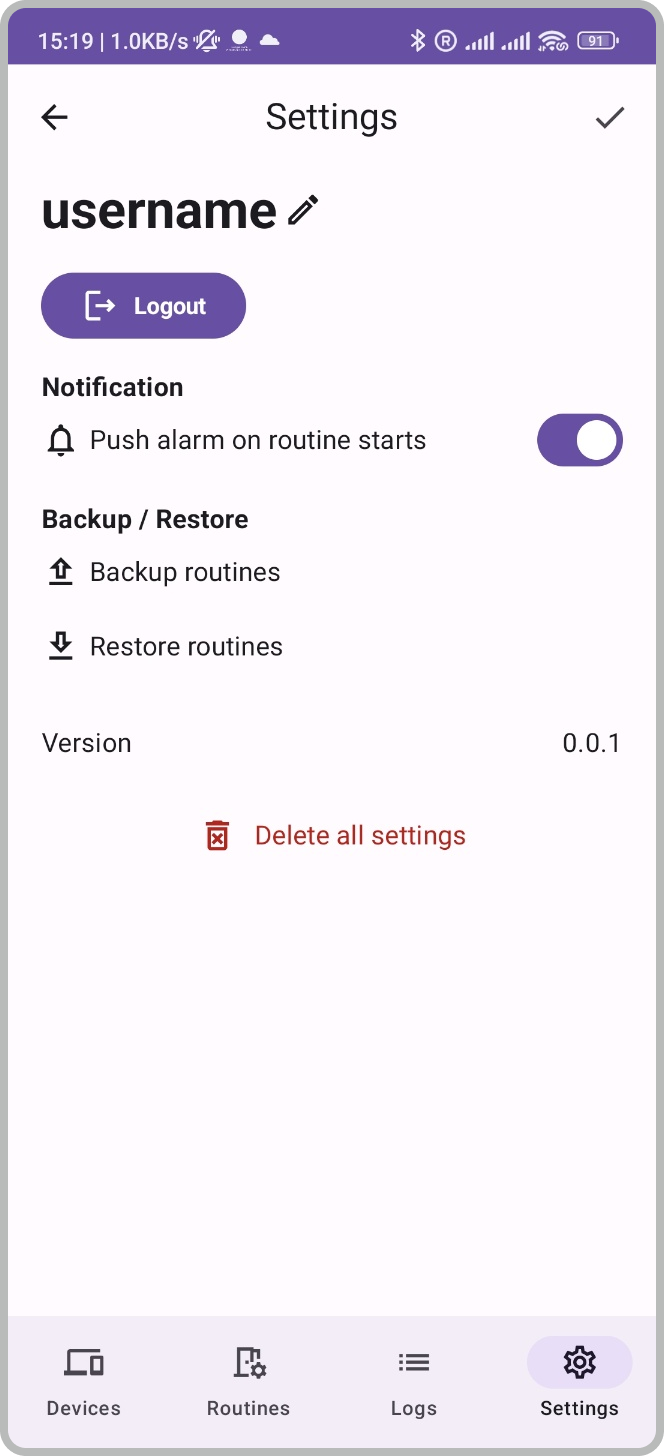
\includegraphics[width=0.5\linewidth]{imgs/usercase/scenario5-a.png}
                        \caption{Scenario 5.a}                        
                    \end{figure}
              \newpage
              \item He can see 'Push alarm on routine starts', and its default status is 'on'.\\
              \item User can change the push notification to the 'off' state by clicking the toggle.\\
                    \begin{figure}[hbt!]
                        \centering
                        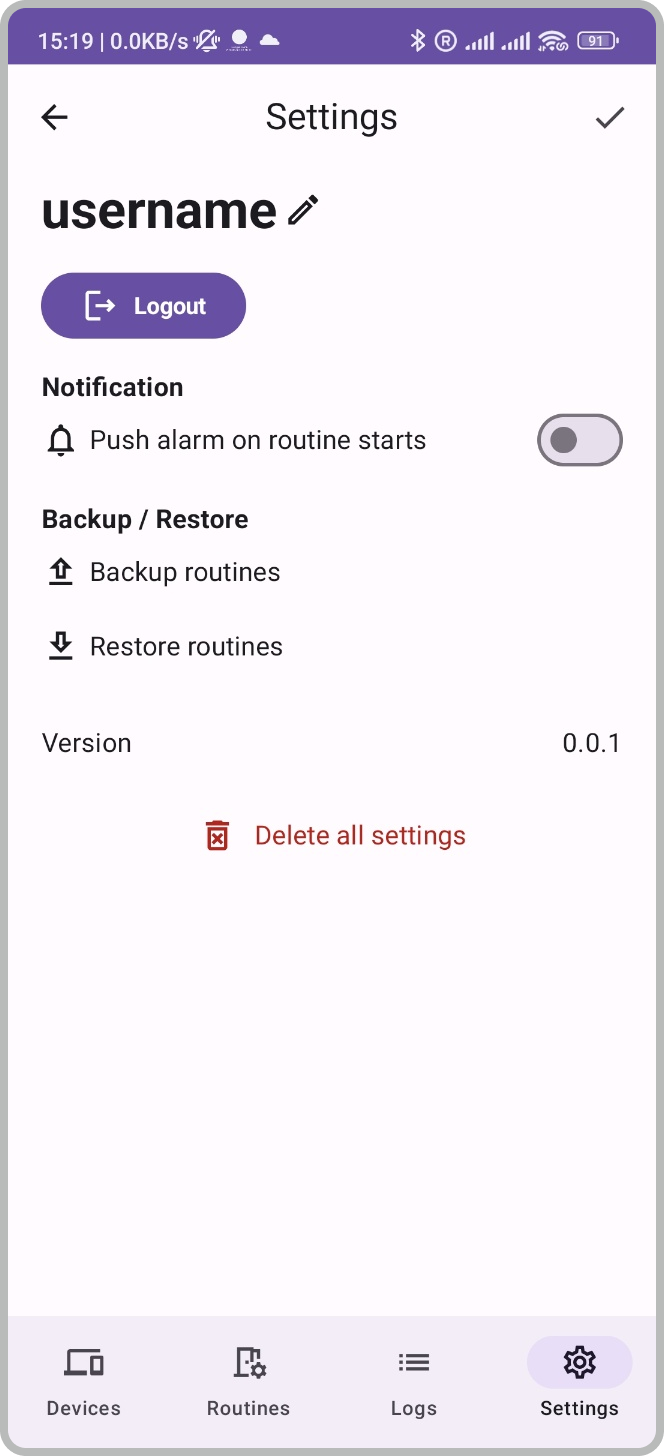
\includegraphics[width=0.5\linewidth]{imgs/usercase/scenario5-c.png}
                        \caption{Scenario 5.c}                        
                    \end{figure}
          \end{enumerate}
          \newpage

    \item Scenario 6\\
          The sixth scenario is to deactivate the 'afternoon routine.' which is activated currently.\\
          \begin{enumerate}
              \item User has to click 'routine' button to bring up the routine page.\\
              \item He can see all routines he created on the page.\\
              \item He should click 'afternoon routine' among the routines to modify its activation setting.\\
                    \begin{figure}[hbt!]
                        \centering
                        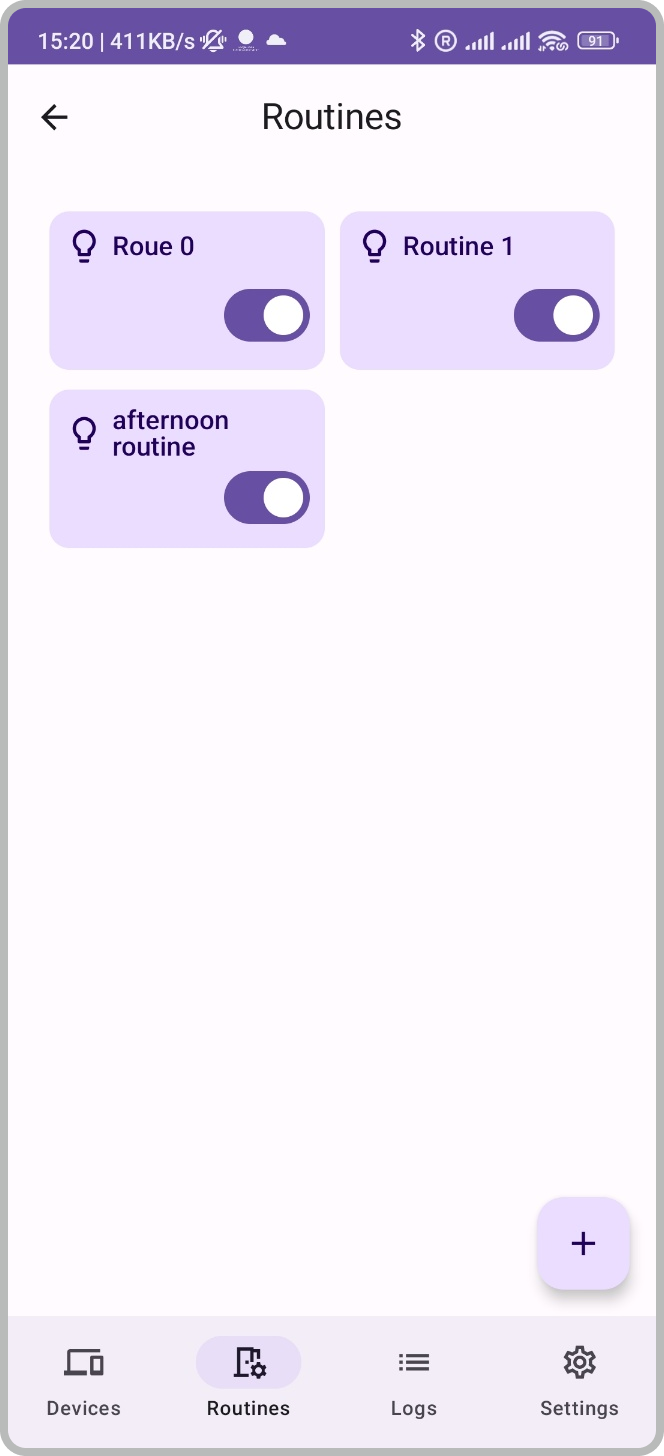
\includegraphics[width=0.5\linewidth]{imgs/usercase/scenario6-a.png}
                        \caption{Scenario 6.c}                        
                    \end{figure}
              \newpage
              \item Then, user can find a toggle next to the routine name.\\
                \begin{figure}[t!]
                    \centering
                    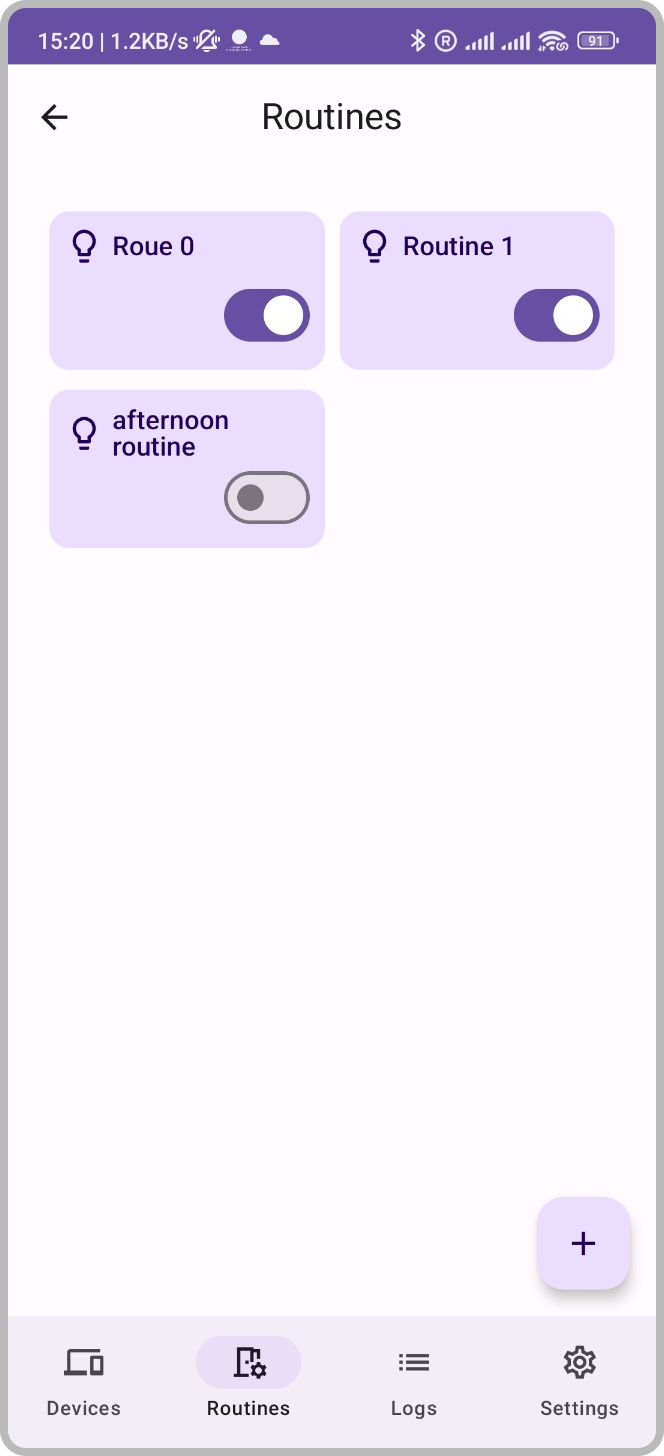
\includegraphics[width=0.5\linewidth]{imgs/usercase/scenario6-c.png}
                    \caption{Scenario 6.e}                        
                \end{figure}
                \newpage
              \item When he click the toggle, the 'afternoon routine' is deactivated.\\
          \end{enumerate}
\end{enumerate}